
This section presents the results obtained in the experiments.

\subsection{The random regression}

I ran the regression input optimization experiment detailed in section \ref{sec:experiments} 25 times. Each experiment was initialized with different random weights on the regression function. For each experiment both optimization methods were allowed to evaluate the function 25 times.

\begin{center}
    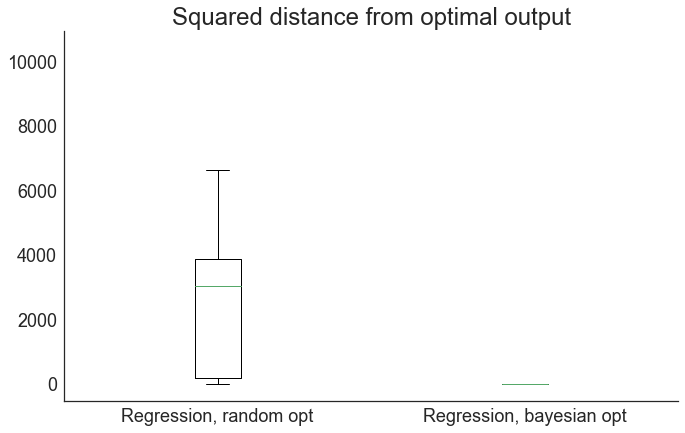
\includegraphics[width=\linewidth]{random_regression.png}
    \captionof{figure}{Squared distance and confidence intervals from the optimal output for both methods. }
    \label{image:random-regression}
\end{center}

\begin{center}
    \begin{tabular}{ c | c | c }
    \bf{Optimization method} & \bf{mean} & \bf{variance} \\
    \hline
    \bf{Random search} & 2925.13 & 8098738.45 \\
    \bf{Bayesian optimization} & 41.42 & 19133.35 \\
    \end{tabular}
    \captionof{table}{Mean squared distance from the optimal output across all 25 runs of the experiments. }
    \label{table:random-regression}
\end{center}

\subsection{Hyperparameter optimization}

Due to the high computational cost of training neural networks, I was only able to run the experiment once for each method. Each method was given 25 function evaluations.

\begin{center}
    \begin{tabular}{ c | c | c }
    \bf{Method} & \bf{best test acc.} & \bf{variance in acc.} \\
    \hline
    \bf{Random search} & 31.23 & 113.98 \\
    \bf{Bayesian optimization} & 31.16 & 98.88 \\
    \end{tabular}
    \captionof{table}{Mean across experiments from the squared distance from the optimum output with the best value found. }
    \label{table:hyperparameter-opt}
\end{center}

The full outputs for the experiments can be seen in appendix \ref{appendix:cnn}



%%% Local Variables:
%%% mode: latex
%%% TeX-master: "report"
%%% End:
